\documentclass[tikz,border=4pt]{standalone}
\usepackage[T1]{fontenc}
\usepackage{lmodern,amssymb}
% stile comune delle figure "da brevetto": bianco e nero, linee sottili, numeri di riferimento
\usetikzlibrary{arrows.meta,calc,patterns,decorations.pathmorphing,decorations.pathreplacing,positioning}
\tikzset{
  every node/.style={font=\scriptsize},
  arr/.style={-{Latex[length=1.8mm,width=1.3mm]}, line width=0.55pt},
  darr/.style={arr, dashed},
  blk/.style={draw, line width=0.6pt, align=center, font=\scriptsize, inner sep=2.5pt},
  thinl/.style={line width=0.35pt},
  figlab/.style={font=\large\bfseries},
}
% \leader{punto}{posizione del numero}{anchor}{numero}
\newcommand{\leader}[4]{\draw[line width=0.3pt] (#1) to[bend left=12] (#2) node[anchor=#3, inner sep=1pt, font=\small]{#4};}

\begin{document}
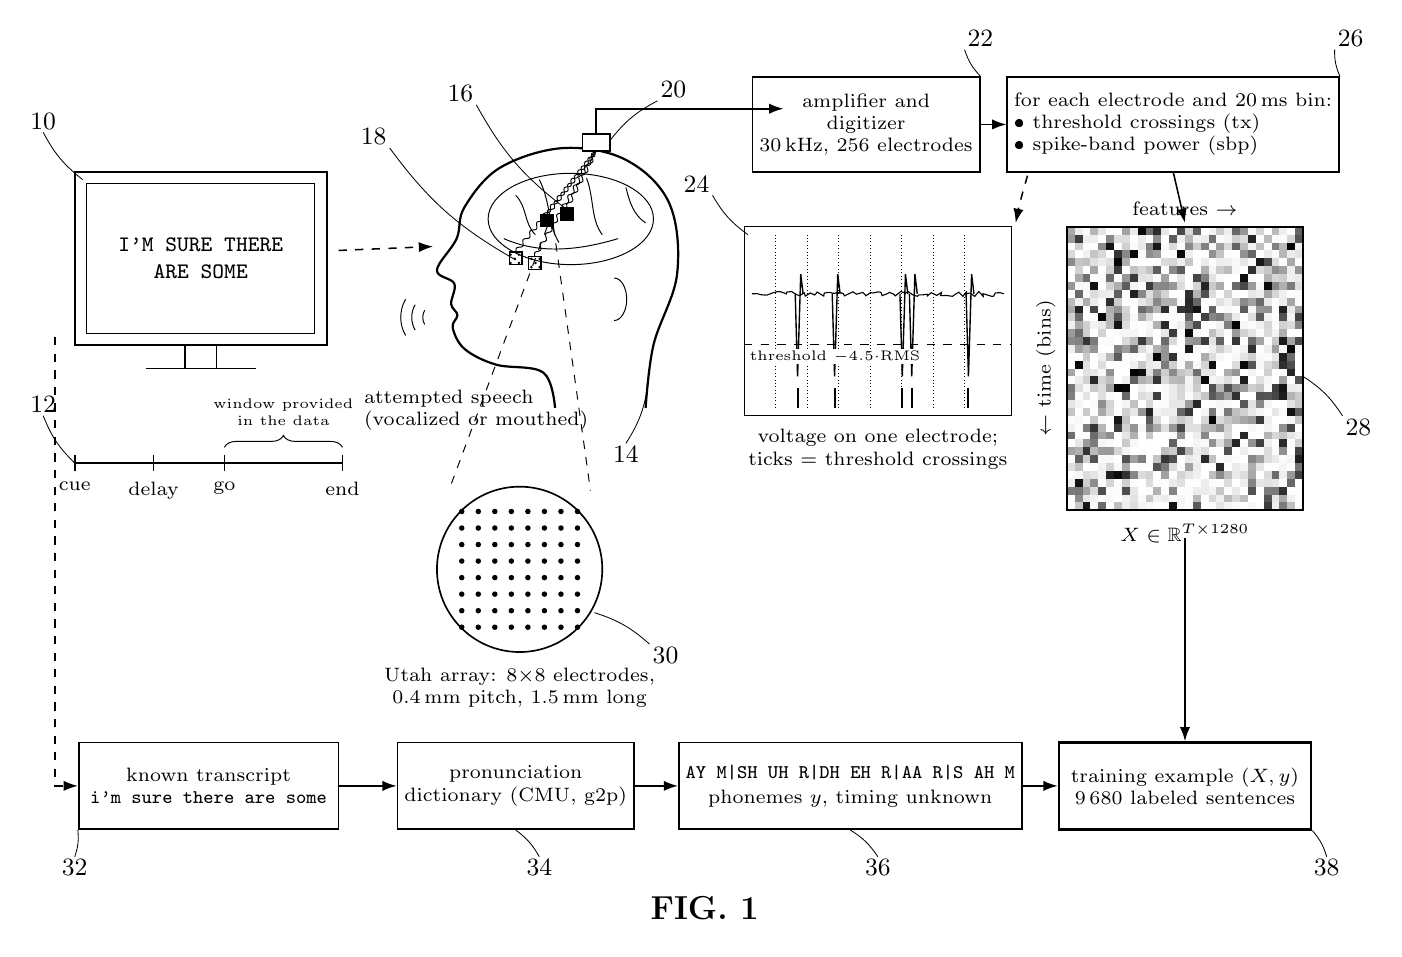
\begin{tikzpicture}[x=1cm,y=1cm]
\pgfmathsetseed{11}

% ---- 10: schermo con la frase ----
\draw[line width=0.8pt] (0,6.4) rectangle (3.2,8.6);
\draw[thinl] (0.15,6.55) rectangle (3.05,8.45);
\node[font=\ttfamily\footnotesize, align=center] at (1.6,7.5) {I'M SURE THERE\\ARE SOME};
\draw[line width=0.6pt] (1.4,6.4) -- (1.4,6.1) (1.8,6.4) -- (1.8,6.1);
\draw[line width=0.6pt] (0.9,6.1) -- (2.3,6.1);
\leader{0.1,8.5}{-0.4,9.1}{south}{10}

% sguardo
\draw[darr] (3.35,7.6) -- (4.55,7.65);

% ---- 14: partecipante (profilo) ----
\draw[line width=0.8pt] plot[smooth, tension=0.6] coordinates {
  (7.25,5.6) (7.35,6.4) (7.65,7.3) (7.55,8.2) (7.0,8.75) (6.2,8.9) (5.4,8.65) (4.95,8.15)
  (4.85,7.75) (4.6,7.35) (4.82,7.18) (4.78,6.92) (4.86,6.78) (4.8,6.62) (4.95,6.35) (5.35,6.15) (5.95,6.05) (6.1,5.6)};
% orecchio
\draw[thinl] (6.85,7.25) arc[start angle=90,end angle=-90,x radius=0.16,y radius=0.27];
% cervello
\draw[thinl] (6.3,8.0) ellipse[x radius=1.05,y radius=0.58];
\draw[thinl] (5.45,7.75) .. controls (5.9,7.55) and (6.4,7.6) .. (6.9,7.75);
\draw[thinl] (5.9,8.5) .. controls (6.05,8.2) and (6.0,7.95) .. (6.15,7.7);
\draw[thinl] (6.5,8.52) .. controls (6.6,8.25) and (6.55,8.0) .. (6.7,7.8);
\draw[thinl] (5.6,8.3) .. controls (5.75,8.15) and (5.7,7.95) .. (5.85,7.8);
\draw[thinl] (7.0,8.4) .. controls (7.05,8.2) and (7.1,8.05) .. (7.25,7.95);
% array: 16 = area 6v, 18 = area 44
\foreach \p in {(5.92,7.9),(6.17,7.98)} \filldraw[fill=black] \p rectangle ++(0.16,0.16);
\foreach \p in {(5.52,7.42),(5.76,7.36)} \draw[pattern=crosshatch dots, line width=0.5pt] \p rectangle ++(0.16,0.16);
\leader{6.25,8.12}{5.1,9.45}{south east}{16}
\leader{5.6,7.48}{4.0,8.9}{south east}{18}
% 20: connettore sul cranio e fili
\draw[line width=0.6pt, fill=white] (6.45,8.86) rectangle (6.8,9.08);
\foreach \s in {(6.0,8.06),(6.25,8.14),(5.6,7.58),(5.84,7.52)}
  \draw[thinl, decorate, decoration={snake,amplitude=0.25mm,segment length=1.4mm}] \s -- (6.62,8.86);
\leader{6.8,9.0}{7.4,9.5}{south west}{20}
% parlato tentato
\foreach \r in {0.18,0.32,0.46} \draw[thinl] (4.6,6.75) ++(150:\r) arc[start angle=150,end angle=210,radius=\r];
\node[align=left, anchor=north west] at (3.55,5.95) {attempted speech\\(vocalized or mouthed)};
\leader{7.28,5.9}{7.0,5.15}{north}{14}

% cavo verso l'amplificatore
\draw[line width=0.6pt] (6.62,9.08) -- (6.62,9.4) -- (8.95,9.4);
\draw[arr] (8.6,9.4) -- (9.0,9.4);

% ---- 22: amplificatore ----
\node[blk, minimum width=2.1cm, minimum height=1.2cm] (amp) at (10.05,9.2) {amplifier and\\digitizer\\30\,kHz, 256 electrodes};
\leader{amp.north east}{11.3,10.15}{south west}{22}

% ---- 26: estrazione feature ----
\node[blk, minimum width=3.7cm, minimum height=1.2cm, align=left] (feat) at (13.95,9.2)
  {for each electrode and 20\,ms bin:\\ \textbullet\ threshold crossings (tx)\\ \textbullet\ spike-band power (sbp)};
\draw[arr] (amp) -- (feat);
\leader{feat.north east}{16.0,10.15}{south west}{26}

% ---- 24: traccia di tensione con soglia ----
\draw[thinl] (8.5,5.5) rectangle (11.9,7.9);
\foreach \x in {8.9,9.3,...,11.7} \draw[densely dotted, line width=0.25pt] (\x,5.6) -- (\x,7.8);
\draw[line width=0.4pt, decorate, decoration={random steps,segment length=0.45mm,amplitude=0.35mm}] (8.6,7.05) -- (11.8,7.05);
\foreach \x in {9.15,9.62,10.48,10.6,11.32} \draw[line width=0.5pt] (\x,7.05) -- (\x+0.03,6.0) -- (\x+0.07,7.3) -- (\x+0.1,7.05);
\draw[dashed, line width=0.4pt] (8.5,6.4) -- (11.9,6.4); \node[anchor=north west, font=\tiny, fill=white, inner sep=0.5pt] at (8.55,6.35) {threshold $-4.5\cdot$RMS};
\foreach \x in {9.18,9.65,10.51,10.63,11.35} \draw[line width=0.7pt] (\x,5.6) -- (\x,5.85);
\node[anchor=north, align=center] at (10.2,5.45) {voltage on one electrode;\\ticks = threshold crossings};
\leader{8.55,7.8}{8.1,8.3}{south east}{24}
\draw[darr] (12.1,8.55) .. controls (12.0,8.2) .. (11.95,7.95);

% ---- 28: matrice X ----
\begin{scope}[shift={(12.6,4.3)}]
\foreach \i in {0,...,29} \foreach \j in {0,...,35} {
  \pgfmathsetmacro{\g}{100*rnd^3}
  \fill[black!\g] (\i*0.1,\j*0.1) rectangle ++(0.1,0.1);}
\draw[line width=0.6pt] (0,0) rectangle (3.0,3.6);
\node[anchor=south] at (1.5,3.62) {features $\rightarrow$};
\node[rotate=90, anchor=south] at (-0.02,1.8) {$\leftarrow$ time (bins)};
\end{scope}
\draw[arr] (13.95,8.6) -- (14.1,7.95);
\leader{15.6,6.0}{16.1,5.5}{north west}{28}
\node[anchor=north, align=center] at (14.1,4.25) {$X\in\mathbb{R}^{T\times 1280}$};

% ---- 12: linea del tempo di una prova ----
\draw[line width=0.6pt] (0,4.9) -- (3.4,4.9);
\foreach \x/\l in {0/cue, 1.0/delay, 1.9/go, 3.4/end} {
  \draw[line width=0.6pt] (\x,4.8) -- (\x,5.0); \node[anchor=north] at (\x,4.78) {\l};}
\draw[decorate, decoration={brace,amplitude=1.5mm}, thinl] (1.9,5.1) -- (3.4,5.1) node[midway, above=1.6mm, align=center, font=\tiny] {window provided\\in the data};
\leader{0,4.9}{-0.4,5.5}{south}{12}

% ---- 30: ingrandimento di un array ----
\draw[thinl, dashed] (6.0,7.9) -- (4.75,4.55);
\draw[thinl, dashed] (6.08,7.9) -- (6.55,4.55);
\draw[line width=0.6pt] (5.65,3.55) circle (1.05);
\foreach \i in {0,...,7} \foreach \j in {0,...,7} \fill (5.65-0.735+\i*0.21, 3.55-0.735+\j*0.21) circle (0.035);
\node[align=center, anchor=north] at (5.65,2.42) {Utah array: 8$\times$8 electrodes,\\0.4\,mm pitch, 1.5\,mm long};
\leader{6.6,3.0}{7.3,2.6}{north west}{30}

% ---- riga in basso: etichetta ----
\node[blk, minimum width=3.3cm, minimum height=1.1cm] (txt) at (1.7,0.8) {known transcript\\\texttt{i'm sure there are some}};
\node[blk, minimum width=2.7cm, minimum height=1.1cm] (dic) at (5.6,0.8) {pronunciation\\dictionary (CMU, g2p)};
\node[blk, minimum width=3.6cm, minimum height=1.1cm] (ph) at (9.85,0.8) {\texttt{AY M|SH UH R|DH EH R|AA R|S AH M}\\[1pt] phonemes $y$, timing unknown};
\node[blk, minimum width=3.2cm, minimum height=1.1cm, line width=1pt] (pair) at (14.1,0.8) {training example $(X,y)$\\9\,680 labeled sentences};
\draw[arr] (txt) -- (dic); \draw[arr] (dic) -- (ph); \draw[arr] (ph) -- (pair);
\draw[arr] (14.1,3.95) -- (pair.north);
\draw[darr] (-0.25,6.5) -- (-0.25,0.8) -- (txt.west);
\leader{txt.south west}{0.0,-0.1}{north}{32}
\leader{dic.south}{5.9,-0.1}{north}{34}
\leader{ph.south}{10.2,-0.1}{north}{36}
\leader{pair.south east}{15.9,-0.1}{north}{38}

\node[figlab] at (8,-0.75) {FIG. 1};
\end{tikzpicture}
\end{document}
